\section{Demonstration}
% Organize this section according to major topics
% give each topic a section heading in boldface.
% try to cover the major common points :
%
% problem design
% methods of measurement
% supporting models
% supporting data
% simulations run
% results

% Just write the section headings for each part and indicate what goes in that
% section with words :
%
% heading
% figures (with captions)
% schematics (with captions and footnotes)
% equations
% tables

% What does it mean?
% What did I actually test?
% What were the results?
% Did the work yield a new method?
% Did the work yield new knowledge?
% What measurements did I make?
% How were these measurements characterized?
% What methods were used?
% What were the results?
% How were the measurements made and characterized?

The early success of the \Cyclus simulator can be measured in many ways. 
The most compelling are demonstrations of the feasibility of the \Cyclus community-driven development 
model and of fundamental simulation capability. Nascent, promising growth of the \Cyclus 
ecosystem at multiple institutions indicates that a fuel cycle simulator can 
advance in a community-driven development paradigm. Simple 
simulations as well as more complex recycling simulations demonstrate that 
\Cyclus possesses fundamental fuel cycle simulation capabilities.

\subsection{Ecosystem}
% Cycamore library
% Cyder?

The \Cyclus `Ecosystem' is the collection of tools, calculation libraries, 
archetypes, data, and input files intended for use with the \Cyclus simulator. 
Members of the ecosystem include:
\begin{itemize}
\item the archetypes provided in the \Cycamore \cite{carlsen_cycamore_2014} 
repository of additional modules,
\item the archetypes created by user-developers,
\item isotopic composition data,
\item historical facility deployment data,
\item the \Cyclus \gls{GUI} tools, Cycic and Cyclist,
\item the tools in the \Cyclus toolkit
\item and other tools for \Cyclus optimization, parallelization, and development.
\end{itemize}
All together, these form an `ecosystem' of capabilities, 
which will grow over time as archetype-developers, kernel-developers, and 
even users contribute capabilities developed for their own needs. Indeed, the 
long-term vision for the \Cyclus framework predicts an ever-expanding ecosystem 
of both general and specialized capability extensions within that ecosystem. 

Already, the ecosystem is growing. Early cross-institutional contributions to 
the ecosystem demonstrate a significant achievement by the \Cyclus framework 
and initiated community-driven development. 

\subsubsection{Supplementary Projects}

A number of projects and tools outside of the core simulation kernel have been 
developed to improve the scope and capabilities of the \Cyclus 
ecosystem. Table \ref{tab:coretools} lists the tools and projects developed 
under close integration with the \Cyclus kernel.
\begin{table}[h]
\centering
\begin{tabularx}{\textwidth}{|r|X|r|}
\hline
\textbf{Name} & \textbf{Description} & \textbf{Citation} \\
\hline
Cycic &  Input control - embedded in Cyclist & \cite{flanagan_input_2013}\\
Cyclist & Interactive data exploration environment & \cite{livnat_cyclist_2014} \\
Ciclus & Continuous Integration scripts for \Cyclus & \cite{scopatz_ciclus_2014}\\
Cycstub & Skeleton for clean slate module development & \cite{carlsen_cycstub_2014}\\
Cyan & \Cyclus analysis tool & \cite{carlsen_cyan_2014}\\
Cloudlus & Tools for running \Cyclus in a cloud environment & \cite{carlsen_cloudlus_2014} \\
\hline
\end{tabularx}
\caption{Many tools outside of the scope of the \Cyclus kernel have been 
developed for improved user, developer, and analyst experiences with \Cyclus.}
\label{tab:coretools}
\end{table}

\subsubsection{Archetype Contributions}

Many archetypes external to the \Cycamore library  
have been 
\cite{huff_streamblender_2014,huff_commodconverter_2014}
and are being 
\cite{flanagan_bright-lite_2014,skutnik_nuclear_2014,huff_mktdriveninst_2014} developed for contribution to the 
\Cyclus ecosystem. These archetypes provide the first examples of 
developer-contributed capabilities.

\begin{table}[h]
\centering
\begin{tabularx}{\textwidth}{|r|X|r|}
\hline
\textbf{Name} & \textbf{Description} & \textbf{Citation} \\
\hline
Bright-lite & A physics-based reactor archetype and fuel fabrication archetype & \cite{flanagan_bright-lite_2014} \\
Nuclear Fuel Inventory Model & A flexible, ORIGEN-based, reactor analysis module & \cite{skutnik_nuclear_2014} \\
CommodConverter & A simple commodity converting storage facility archetype  & \cite{huff_commodconverter_2014} \\
MktDrivenInst & An institution that controls deployment based on commodity availability & \cite{huff_mktdriveninst_2014} \\
SeparationsMatrix & A facility for elemental separations of used fuel & \cite{huff_streamblender_2014} \\
StreamBlender & A facility for fuel fabrication from reprocessed streams & \cite{huff_streamblender_2014} \\
\hline
\end{tabularx}
\caption{The range of  archetypes under development reflect the diverse 
needs of researchers at various institutions. These archetypes, contributed 
outside of the \Cyclus core and \Cycamore libraries are the first demonstration 
of community-driven development in a fuel cycle simulator.}
\label{tab:archetypes}
\end{table}


\subsection{Simulations}
%Inpro example (is this still running or did we deprecate it with 1.0?)

% MJG - INPRO should be tried again. @rwcarlsen has been running lots of
% simulations with the batch reactor, and its the second generation of my
% reactor models. We could easily use the same demand schedule and enrichment
% facility parameters and run it again.

Results of some simple recycle scenarios simulated via \Cyclus follow.  In \Cyclus,
because material is tracked as discrete objects, single-pass MOX recycle is
easy to implement.  The simulation duration was 1100 months and included one
of each of the following: fresh
UOX fuel fabrication, recycled MOX fuel fabrication, reactor, separations
facility, and repository.

The \Class{BatchReactor} archetype from \Cycamore accepts
fuel materials from an arbitrary number of sources delineated by
commodity. Custom, non-uniform preferences can be set for each fuel
commodity.  The \gls{DRE} enables reactors to
preferentially accept recycled MOX fuel over fresh UOX fuel.  The
\Class{BatchReactor} was configured with a 3-batch core on 18-month cycles and
a 2-month refueling period.  Adjusting and setting parameters such as these
simply requires editing input file numbers, as shown below:

\begin{lstlisting}[language=xml]
  ...
  <BatchReactor>
      ...
      <processtime>18</processtime>
      <nbatches>3</nbatches>
      <batchsize>20000</batchsize>
      <refueltime>2</refueltime>
      ...
  </BatchReactor>
  ...
\end{lstlisting}

The \Class{Source} and \Class{Sink} modules from \Cycamore were chosen to be a
source of fresh, enriched uranium and a repository, respectively. The simple
recycled fuel fabrication facility was designed to
mix fissile and fertile streams to match target fuel compositions as closely
as possible.  The method used for this matching is similar to
that used by the \gls{COSI} fuel cycle simulator \TODO{cite COSI equivalence
method}. The material flows for this simulation are shown below in Figure
\ref{fig:flowmodopen}.

\begin{figure}[H]
\begin{center}
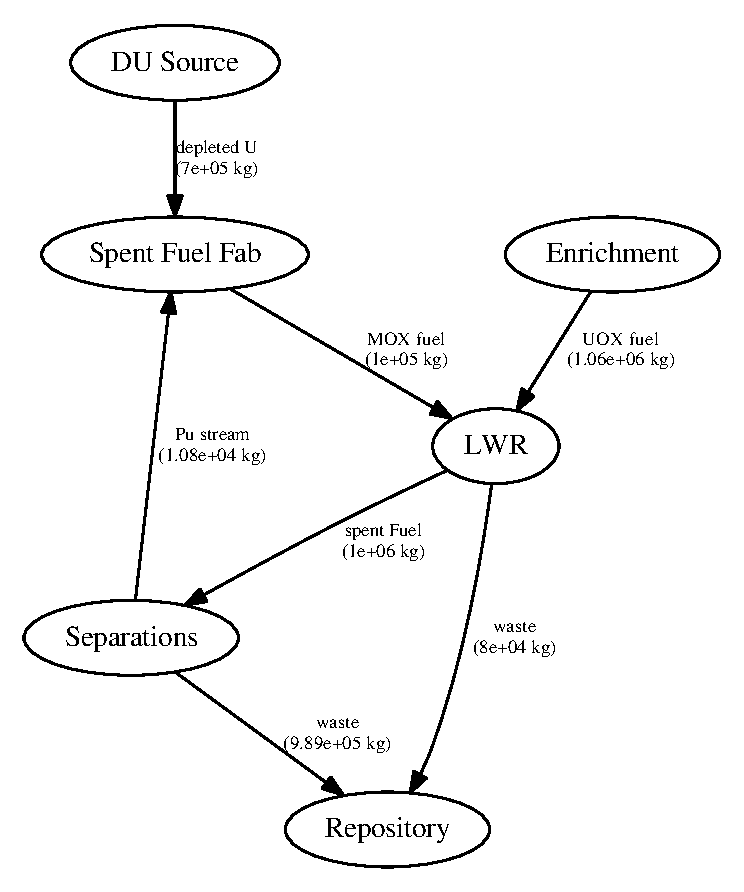
\includegraphics{./images/flow-mod-open-1.eps}
\end{center}
\caption{Modified open 1-pass MOX recycle fuel cycle material flows.}
\label{fig:flowmodopen}
\end{figure}

Simply changing the output commodity name of spent MOX fuel from the 
\Class{BatchReactor} transforms this simulation into a closed fuel cycle.
The one-word change in the input file is shown below: 

\begin{lstlisting}[language=diff]
  --- mod-open-1.xml	2014-10-08 08:31:33.892523173 -0500
  +++ closed-1.xml	2014-10-08 08:31:33.892523173 -0500
  @@ -108,7 +108,7 @@
           <fuel>         
             <incommodity>mox_fuel</incommodity>
             <inrecipe>lwr_mox_fuel</inrecipe>
  -          <outcommodity>spent_mox</outcommodity>
  +          <outcommodity>spent_fuel</outcommodity>
             <outrecipe>mox_spent_fuel</outrecipe>
           </fuel>
\end{lstlisting}

This new simulation results in the material flows seen in Figure \ref{fig:flowclosed}. Note
that because the \Class{BatchReactor} always transmutes fuel into the same
composition, the nuclide level flows are not accurate for the full, 
multi-pass
recycle case.

\begin{figure}[H]
\begin{center}
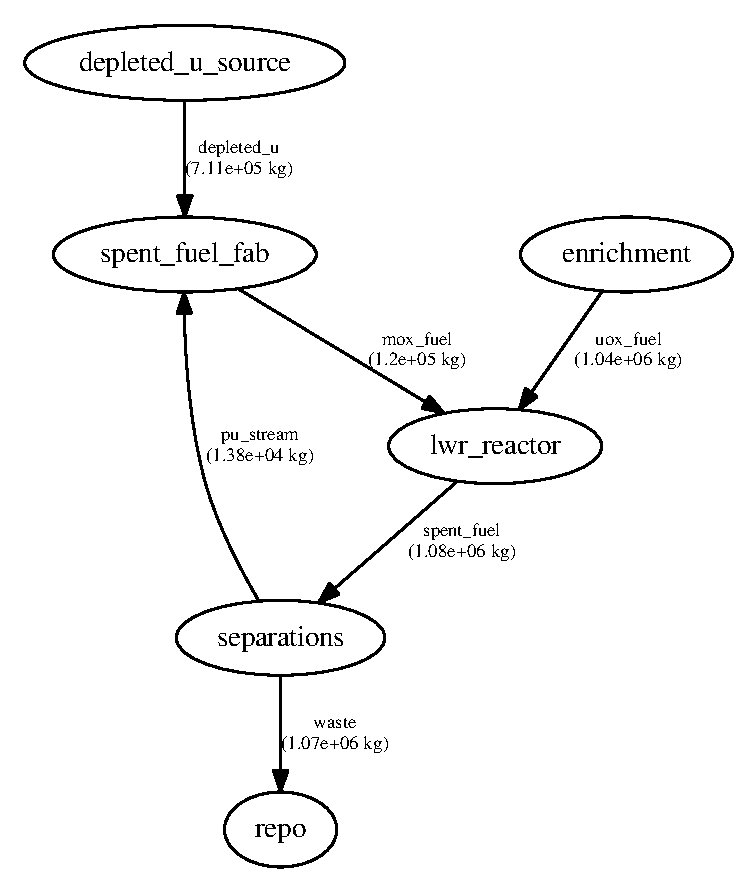
\includegraphics{./images/flow-closed-1.eps}
\end{center}
\caption{Full MOX recycle (multi-pass) fuel cycle material flows.}
\label{fig:flowclosed}
\end{figure}

Figure \ref{fig:puseries1} shows the full-system plutonium buildup for open
(no recycle), modified open, and closed (infinite-pass recycle) variations of
the single-reactor scenario described above.  The figure was
generated directly from \Cyclus output data. After several batch cycles (near
month 300) in both the modified open and closed cases, enough separated fissile
material accumulates in the fuel fabrication facility to generate a full
recycled batch.  When this batch is transmuted, more plutonium is burned than
created.  This results in a drop in the total fuel cycle system plutonium
inventory.  This pattern repeats roughly every 10 cycles (200 months) for the
modified open case and every 9 cycles (180 months) for the closed case.
Because the modified open scenario does not re-recycle material, the
fabrication facility takes 1 additional cycle to accumulate a full batch of
fissile material.  Because facilities are represented individually and
transact materials as discrete events, realistic non-uniform patterns
in facility behavior can be observed that affect total system behavior in ways
less commonly observed in fleet-based, continuous material flow
modeling.

\begin{figure}[H]
\begin{center}
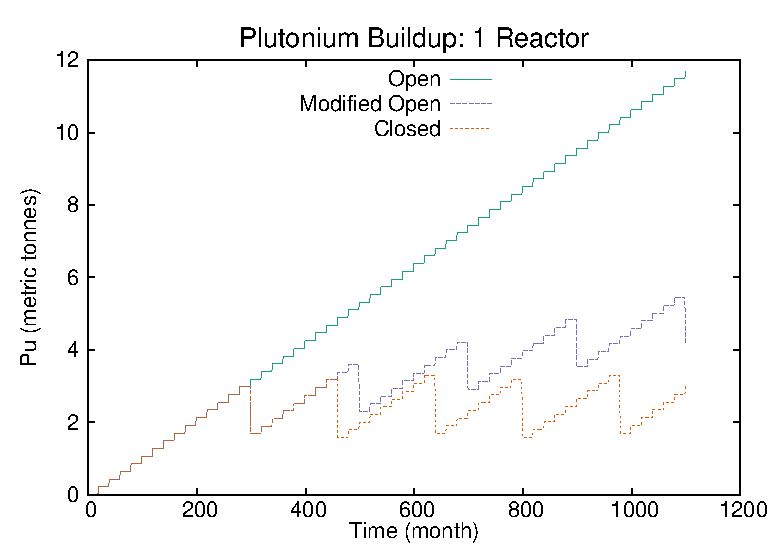
\includegraphics{./images/puseries-1.eps}
\end{center}
\caption{System plutonium buildup with one reactor.}
\label{fig:puseries1}
\end{figure}

The open, modified open, and closed scenarios can easily be configured to
stagger the refueling times of the reactors.  As the number of
reactors increases, the behavior of the system approaches an average behavior,
reminiscent of continuous material flow models.  The plutonium buildup
for these three multi-reactor variations is shown in Figure
\ref{fig:puseriesn}.

\begin{figure}[H]
\begin{center}
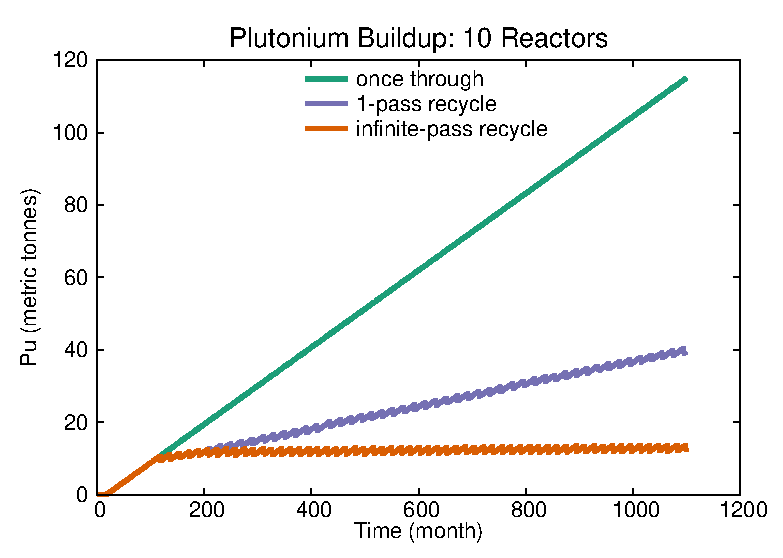
\includegraphics{./images/puseries-n.eps}
\end{center}
\caption{System plutonium buildup with staggered refueling for many reactors.}
\label{fig:puseriesn}
\end{figure}

